\section{Introduction}

\begin{frame}{MOTIVATION}
    \begin{itemize}
        \item Most IoT devices operate with constrained computational capabilities and limited resources.
    \end{itemize}
    \begin{table}[ht]
    \scriptsize
    \caption{Classification of IoT devices based on hardware capabilities.}
    \begin{tabular}{@{}llllll@{}}
    \toprule
    \textbf{Category} & \textbf{CPU} & \textbf{RAM} & \textbf{Storage} & \textbf{Power} & \textbf{Example} \\ 
    \midrule
    Category 1 & 8-bit, 16 MHz & $\leq$ 32 KB & Small & $\leq$ 1 W & Arduino Mega \\
    Category 2 & 32-bit, 80 MHz & 32–80 KB & Small & $\leq$ 1 W & NodeMCU ESP-12 \\
    Category 3 & Single-core, 1 GHz & 80 KB–512 MB & $\leq$ 4 GB & 1–2 W & Raspberry Pi Zero \\
    Category 4 & Quad-core, 1.2 GHz & 512 MB–2 GB & $\leq$ 8 GB & 2–4 W & Raspberry Pi 3 \\
    Category 5 & Quad-core, 2 GHz & $\geq$ 8 GB & $\geq$ 32 GB & High & Jetson TX2 \\
    \bottomrule
    \end{tabular}
    \end{table}
\end{frame}

\begin{frame}{MOTIVATION}
    \vspace{0.5cm}
    \begin{itemize}
        \item Most IoT devices operate with constrained computational capabilities and limited resources.
    \end{itemize}
    \begin{figure}
        \centering
        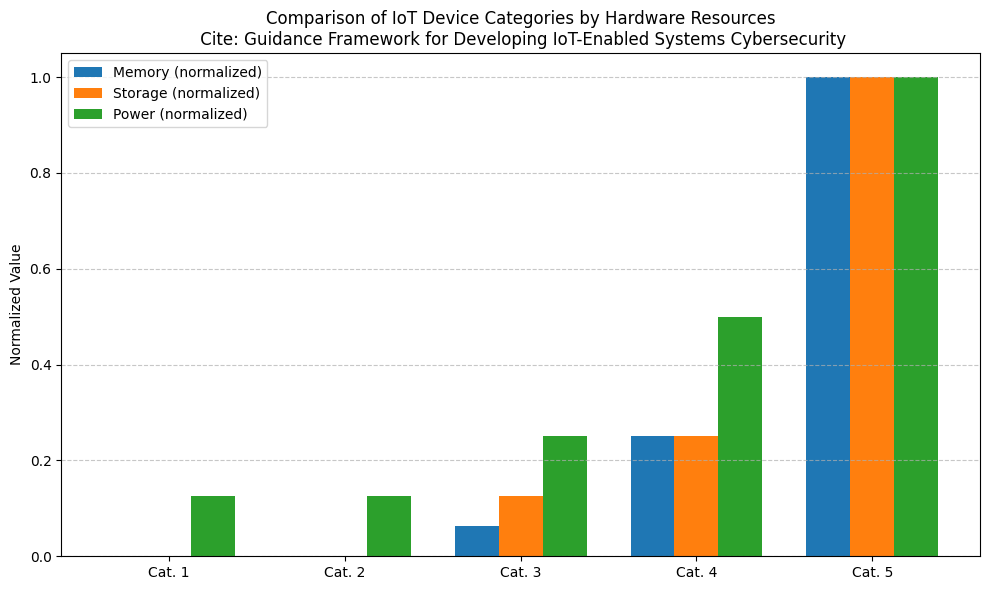
\includegraphics[width=0.65\textwidth]{pic/cat.png}
    \end{figure}
\end{frame}

\begin{frame}{MOTIVATION}
    \begin{columns}
        \begin{column}{0.45\textwidth}
            \begin{itemize}
                \item Research on implementing complete IoT architectures remains limited.
            \end{itemize}
        \end{column}
        \begin{column}{0.55\textwidth}
            \centering
            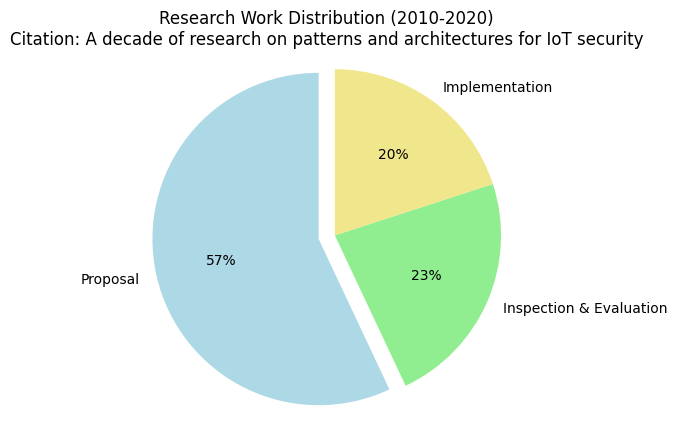
\includegraphics[width=1\linewidth]{pic/research2.png}
        \end{column}
    \end{columns}
\end{frame}

\begin{frame}{Objectives and Contributions}
This work aims to develop a complete IoT architecture that fulfills the following goals:
\begin{enumerate}
    \item Compatible with a \textbf{wide range} of hardware platforms.
    \item Ensures \textbf{data integrity} and \textbf{confidentiality} during transmission.
    \item Provides mechanisms to \textbf{mitigate common attacks}.
    \item \textbf{Implementation} on real hardware and performance benchmarking.
    \item Can be used as a \textbf{reference} framework for future IoT implementations.
\end{enumerate}
\end{frame}
